\documentclass[11pt,a4paper]{article}

\usepackage{hyperref}
\usepackage{graphicx}
\usepackage{amssymb}
\usepackage{amsmath}
\usepackage{amsthm}
\usepackage[margin=19mm]{geometry}
\usepackage{natbib}
\usepackage{bm}
\usepackage[toc,page]{appendix}
\usepackage{booktabs}
%\usepackage{url}
%\usepackage{fancyhdr}
%\usepackage{fancyvrb}
\usepackage{lscape}
%\usepackage{pdfsync}
\usepackage{rotating}
\usepackage{multirow}
\usepackage[nodisplayskipstretch]{setspace} \setstretch{1.5}
\let\oldv\verbatim
\def\verbatim{\par\setstretch{0.9}\oldv}
\usepackage[table]{xcolor}
\usepackage{algorithm,algorithmic}

%\renewcommand{\headrulewidth}{0.5pt} %Do not print a rule below the header
%\renewcommand{\footrulewidth}{0pt} %Do not print a rule above the footer

\bibpunct{(}{)}{;}{a}{,}{,}

%\renewenvironment{tabbing}{\linebreak \texttt \sl}{\linebreak}

\newcommand{\undertilde}[1]{\underset{\widetilde{}}{#1}}
\newcommand{\threeScript}[3]{
	\!\begin{smarray}{l}
  		{#1}\\ \hlx{s[-5pt]}
  		{#2}\\ \hlx{s[-5pt]}
  		{#3}
 	 \end{smarray}
}
\renewcommand{\baselinestretch}{1.5}
\setlength{\abovecaptionskip}{5pt}
\setlength{\belowcaptionskip}{-1pt}

\newtheorem{mydef}{Definition}

\floatname{algorithm}{Pseudocode}

\newcommand{\disfrac}{\displaystyle \frac}

\hypersetup{
    bookmarks=true,         % show bookmarks bar?
    unicode=false,          % non-Latin characters in Acrobat’s bookmarks
    pdftoolbar=true,        % show Acrobat’s toolbar?
    pdfmenubar=true,        % show Acrobat’s menu?
    pdffitwindow=false,     % window fit to page when opened
    pdfstartview={FitH},    % fits the width of the page to the window
    pdftitle={My title},    % title
    pdfauthor={Author},     % author
    pdfsubject={Subject},   % subject of the document
    pdfcreator={Creator},   % creator of the document
    pdfproducer={Producer}, % producer of the document
    pdfkeywords={keyword1} {key2} {key3}, % list of keywords
    pdfnewwindow=true,      % links in new window
    linktoc = page,
    colorlinks=true,       % false: boxed links; true: colored links
    linkcolor=blue,          % color of internal links
    citecolor=blue,        % color of links to bibliography
    filecolor=magenta,      % color of file links
    urlcolor=cyan           % color of external links
}

%###################################################################################################
%Writing starts here!!
%
%###################################################################################################

\begin{document}
\title{Introduction}
\author{Kevin Chang}
\date{\today}
\maketitle

%\tableofcontents
%\chapter{Introduction}\label{chap:intro}

\section{Introduction}
All research studies require that the researchers conduct one or more experiments to make confident claims to support or refute a particular hypothesis based on the study results. A carefully thought out plan for an experiment is essential, and is an important discipline of study called \emph{experimental design}. The initial foundations of statistical approach to design the experiments were laid by \cite{Fisher1935} in the field of agriculture, but it is now applicable to almost all sciences. \citeauthor{Fisher1935}'s main focuses were in the principles of comparison, randomisation, replication, blocking, orthogonality and the use of factorial treatments in connection with the design of experiment. These concepts should be implemented in a carefully thought out experiment if the researcher wishes the result to stand up to scrutiny.


Carefully thought out experimental design offers several advantages. First, it increases the information obtained per experiment versus an ad hoc approach, because a carefully planned experiment can protect against confounding of the effects of interest from nuisance sources of variation. Further, a good experiment provides an organised approach to conduct the experiment, to analyse the data sets and to interpretation the results. Thus, the findings from the experiment should be reproducible, which facilitates the communication between statisticians and researchers  \citep{Doyle2009}. 

%However, most of these principles were developed without or with only minimal computational power, and views on experimental design have changed considerably since the 1930s \cite{John1987}. Theories of experimental design have developed particularly rapidly with advances in computers. 
 
 
This thesis focuses on \emph{high-throughput biotechnologies experiment} (HTBE). HTBE involves the simultaneous testing of multiple samples in a biological assay, where each sample comprises large numbers of candidate molecules, such as genes or proteins \citep{Janzen2002}. Thorough experimental design is particularly important in HTBE owing to the high cost of such experiments. However, while high-throughput biotechnologies have improved rapidly over the last decade, statistical methods for analysing data generated from these technologies have failed to keep up \citep{Doyle2009}. Therefore, theories related to the design of HTBE need improvement. 

For most HTBE, the responses of the experimental units to treatments cannot be measured directly in a single experiment, e.g.\ the gene expression level cannot be measured without using microarray technology. Thus, subsequent processing (Phase 2) of the results of the initial (Phase 1) experiment is necessary to obtain useful measurements. Another example is a proteomics experiment, which involves the study of proteins. The Phase 1 experiment involves the organisms to be perturbed by the experimental conditions of interest. Since the abundance of proteins cannot be measured directly from the organisms, the Phase 2 experiment is required to measure the abundance of proteins in samples extracted from the organisms in the Phase 1 experiment. An example of the Phase 2 experiment is the application of a multiplexing technique such as iTRAQ peptide labelling, coupled with liquid chromatography-mass spectrometry (LC-MS). Section~\ref{sec:proteomicExpt} details the biological background of the mass spectrometry based proteomics experiments. 

This chapter establishes a general understanding of the two-phase experiments. Section~\ref{sec:introTwoPhase} to \ref{sec:brien2011} then describes how the methods surrounding the two-phase experiments have evolved over recent decades. The biological background of proteomics experiments is then explained in Section~\ref{sec:proteomicExpt}. Finally, Section~\ref{sec:overview} presents a brief overview of this thesis.


\section{The introduction of two-phase experiments by McIntyre}
\label{sec:introTwoPhase}
Two-phase experiments were first introduced by \cite{McIntyre1955}, who used a real example involving the investigation of the effects of four light treatments on the synthesis of tobacco mosaic viruses in tobacco leaves. In the Phase 1 experiment, two $4 \times 4$ square arrays are made up by eight plants and four leaves within plants. Four different treatments are then assigned to the plants and leaves such that each treatment occurs only once within each row and column in each of two $4 \times 4$ square arrays. This assignment is also known as \emph{Latin square design} \citep{Bailey2008}. The Phase 1 experiment thus yielded 32 observations. However, the virus contents from each leaf cannot be measured directly in the Phase 1 experiment. Hence, the virus content of the leaves from the plants used in the Phase 1 experiments, referred to as the \emph{test plants}, was assayed by expressing sap using a completely different set of plants, referred to as the \emph{assay plants}, for the Phase 2 experiment. 

The Phase 2 experiment used four leaves from each of 16 assay plants. Each leaf was further subdivided into two halves, thus allowing the measurement of 128 samples. Given that the Phase 1 experiment involved 32 samples, each sample was replicated four times in the Phase 2 experiment. For the assignment of the Phase 2 experiment, four $4 \times 4$ square arrays are made up using the four leaves from each of 16 plants. Since each leaf was further divided into two halves, the Phase 2 design can be expressed as two sets of Latin square designs superimposed on each other, an arrangement also known as the \emph{Greaco-Latin square design}. This experiment provides a good example of a two-phase experiment that requires two different experimental designs, where the first design prepares a set of samples and second design measures bio-substances of interest from each sample. 

The analysis of variance (ANOVA) table explained the sources of variation introduced from the two-phase experiment. For each source of variation, the \emph{sum of squares} (SS) can be computed from the experimental data and the \emph{expected mean squares} (EMS) can be derived solely from the experimental design. EMS is the linear combination of \emph{variance component}, commonly denoted by $\sigma_{i}^2$ from factor $i$, which indicates the contribution of the variation from different factors. The ANOVA table thus is essential for identifying and analysing the variations among experiments, and can useful for complex experiments involving many factors, such as two-phase experiments. 

\cite{McIntyre1955} presented two important principles in the design of the two-phase experiment. The replication of the treatment in the Phase 1 experiment is essential, because the statistical test of the treatment effects for the Phase 1 experiment should be achievable separately from the Phase 2 experiment. Replication in the Phase 2 experiment is unnecessary unless the experiment introduces uncontrollable variation. The main theoretical objective of the two-phase experiment is to identify the relationship between the factors from the Phase 2 and Phase 1 experiments. For the example mentioned above, the treatments are replicated four times in Phase 1. Additionally, each sample from the Phase 1 experiment is further replicated four times before being assigned to the Phase 2 experiment. 

\cite{McIntyre1955} concluded by identifying three important concepts. First, he demonstrated that the different two-phase design combinations can induce different error variances for the treatment effects, because different designs cause different combinations of the variance components. Second, based on the example experiment, given doubling in the replication in the Phase 2 experiment, the error variance for the treatment effects is reduced by only $19\%$, but the time required to complete the experiment is doubled. Third, the absence of treatment replication within the Phase 1 experiment inflates the error variance for the treatment effects. This is because the error variance includes the variation among leaves from single plants from both the Phase 1 and Phase 2 experiments. 

To summarise, the construction of the ANOVA table with EMS is shown to be essential to illustrate the linear combination of the variance components because it allows the estimation of the error variance for the treatment effects. However, the method used to construct the ANOVA table with EMS was not mentioned by \cite{McIntyre1955}.
 
\section{Non-orthogonal structure of the two-phase experiment}
\cite{Curnow1959} revisited the theory of two-phase experiments and produced a new ANOVA table presenting an overall analysis of the light treatment experiment from \citeauthor{McIntyre1955}. The new ANOVA table is better than that presented by \cite{McIntyre1955}, because it shows every SS and the corresponding \emph{degrees of freedom} (DF) for the light treatment experiment. Additionally, the ANOVA table also shows the separation of the treatment effects according to source of variation. The first estimate of treatment effects contains the variance components between leaves from the assay plants, whereas the second estimate does not. \cite{Curnow1959} labels these first and second estimations of the treatment effects as \emph{sums} and \emph{differences} analyses, respectively, which are equivalent to \emph{inter} and \emph{intra}-block analyses, respectively. \cite{Curnow1959} then showed how to combine the inter- and intra-block analyses using the weights computed from the variance of treatment estimate. Nevertheless, the new ANOVA table, given by \cite{Curnow1959}, emphasised the combination of estimates from the intra- and inter-block analyses, which provides a first step towards developing a better analytical procedure for the two-phase experiments. 

\cite{Wood1988} then discussed the non-orthogonal block structure of the two-phase experiments, which is an extension of the theory described by \cite{Curnow1959}. The \emph{block structure} is the relationship between the block factors, and hence the \emph{treatment structure} is the relationship between the treatment factors. The non-orthogonal structure typically occurs when the treatment effects can be estimated from both inter- and intra-block analyses, as in the examples from \cite{McIntyre1955} and \cite{Curnow1959}, i.e.\ non-orthogonal treatment structure. Similarly, the non-orthogonal block structure can also occur when the block factor from the Phase 1 experiment is confounded with that from the Phase 2 experiment for the two-phase experiment. The orthogonality can be measured by the \emph{efficiency factor} which is the amount of treatment information presented for the intra-block analysis \citep{Yates1936}. Thus, the efficiency factor should also be used to measure the block information for cases involving non-orthogonal block structure. 

Non-orthogonal structure has two different origins. The first is that the DF of block effects from the Phase 1 experiment are split into inter- and intra-blocks. This can be shown in the ANOVA table given by \cite{Curnow1959} where the total of 6 DF associated with the leaf positions of the test plants is split into 2 SS, where both SS are estimated with 3 DF. This first SS is confounded with the whole leaves of the assay plants and the second is orthogonal to them. The efficiency factor for both SS can be shown to be 100\%. The second origin is that the DF of block effects from the Phase 1 experiment remain intact. This can be shown in the artificial example by \cite{Wood1988} where all three DF associated with the units SS of the Phase 1 experiment are estimated both Between and Within Blocks. The separation for this case is then measured using the efficiency factor. Both types of confounding should be minimised, because they can affect on how the test for the treatment effects is conducted. Chapters 3 and 4 describe the findings regarding the optimal two-phase design, and further discuss the non-orthogonal treatment and block structures. 

\section{Constructing the analysis of variance table}
Neither the \cite{McIntyre1955} nor \cite{Curnow1959} mentioned how their ANOVA tables were determined, particularly for complex experiments such as two-phase experiments. \cite{Brien1983} thus presented a generalised procedure for determining the ANOVA table. Notably, the presented ANOVA consists only of sources of variation and the corresponding DF. This section briefly describes the procedure presented by \cite{Brien1983}, which contains some basic terminologies of experiment design.

Before constructing the ANOVA table, the overall structure of the experiment must be determined. The first step is to identify the factors in the experiment and the observational unit. The observational unit is the smallest unit of the experiment \cite{Bailey2008}. Meanwhile, the second step is to divide the factors into different sets, also known as \emph{tiers}. The first tier consists of the factors that jointly identify the observational unit in the absence of randomisation. \cite{Nelder1965A} also labelled these factors block factors. The second tier factors are those level combinations that are directly associated with those of the factor at the first tier, and are usually known as \emph{randomisation}. Thus, \cite{Nelder1965B} labels the second tier factors treatment factors.
 
The last step is to determine the relationship between the factors within each tier. \cite{Wilkinson1973} developed a symbolic syntax for representing the block and treatment structures in an experiment. \cite{Brien1999} termed this representation a \emph{structure formula}. \citeauthor{Wilkinson1973}'s syntax was originally developed to generate and analyse the ANOVA models in the GenStat statistical analysis program, although it is now widely used in many statistical packages. Two basic operations described by \cite{Wilkinson1973} are used to represent block and treatment structures, namely \emph{crossing} denoted by an asterisk, $*$, and \emph{nesting}, denoted by a slash, $/$. 

The two-phase experiment involves three tiers of factors, two sets of block factors and one set of treatment factors. Consequently, two-phase experiments are also known as \emph{multi-tiered experiments}. Tiers 1 and 2 comprise block factors from the Phase 2 and 1 experiments, respectively. Tier 3 contains the treatment factors of the overall experiments.  

The ANOVA table can be obtained once the structural formula for every tier of the experiment is determined. The first step is to expand the structure formulae for each tier, which yields a set of terms based on the rules described by \cite{Wilkinson1973}. The terms from the first tier form an initial structure of the ANOVA table. Meanwhile, the terms from the second tier are included in the table under the terms of the first tier with indentation, and only if the two terms from different tiers are confounded. The confounding between the terms can be examined using the contrasts generated from each term. The two-phase experiment includes an additional tier. Therefore, the terms from tier 3 are grouped with those of tiers 1 or 2, with another indentation if confounding occurs between the terms from the two different tiers. For a more detailed description of these procedures see \cite{Brien1983}.

\cite{Brien1983} concluded by expressing the idea that the randomisation between the factors of different tiers can alter the relationships among factors within each tier. Consider an experiment arranged by the row-column design, then the relationship between the row and column factors should \emph{crossed}. However, if the treatment factor can only be randomised to the column factor, then it becomes confounded with the column factor. Consequently, the relationship between the row and column factors becomes \emph{nested}. To summarise, the experimental structure depends on both the innate physical structure and on how the randomisation is employed. 

\section{Complicated two-phase experiments}
The rules described in \cite{Brien1983} can be difficult to apply to a complicated two-phase experiment with non-orthogonal structure. This is because the confounding between the terms of different tiers can be hard to examine using their contrasts alone. \cite{Brien1999} thus described an algorithm that fits terms into the model using two types of sweeping operations.  The algorithm can construct the ANOVA table for any single- or two-phase experiment. 

The sweeping operations were originally discussed by \cite{Wilkinson1970} and \cite{Payne1977}. The first sweep operator is the \emph{pivotal sweep} which involves the effects placed in a unit length vector. The data vector thus is projected from one vector subspace to another, where each vector subspace corresponds to each term expanded from the structure formula. This sweeping operator thus can be expressed as 
\begin{equation}
E_i \mathbf{Q}_i
\end{equation}
where $E_i$ and $\mathbf{Q}_i$ are the efficiency factor and orthogonal projector matrix associated with term $i$ from the expanded structure formula. The second sweep operator is called \emph{reanalysis sweep}. This sweep is performed on terms with two different structural formulae that are non-orthogonal, i.e.\ non-orthogonal block or treatment structures. Hence, before performing the pivotal sweep during the next term, the effect of the current term is removed using the reanalysis sweep. This sweeping operator can be expressed as 
\begin{equation}
\mathbf{I} - E_i \mathbf{Q}_i
\end{equation}
where $\mathbf{I}$ is the identity matrix. Since the methods are based on vector projection, the reanalysis sweep is based on the \emph{Pythagorean theorem}, which involves the subtraction of two vectors to obtain the resultant vector with orthogonal complement.

\cite{Brien1999} addressed that this algorithm can be extended for the two-phase experiment by performing additional sweeps for terms from the third structure formula. These two sweeping operators are vital to the decomposition of the raw data and the computation of the SS for the ANOVA table. This is further discussed in Chapter 2.

\section{Moving toward the high-throughput biotechnology}
\cite{Jarrett2008} demonstrated how the two-phase experiment can be applied to the gene expression two-colour microarray experiments. The Phase 1 experiment requires an experimental design to prepare the two additional conditions for comparison. This experiment then provides some physical materials, i.e.\ mRNA, for the Phase 2 experiment. Another experimental design is required for the Phase 2 experiment dealing with how the samples from the Phase 1 experiment are allocated to different dyes and arrays. The Phase 2 experiment ultimately generates numerical values that need to be analysed. 

\cite{Jarrett2008} demonstrated how to assess the effectiveness of the estimates using the effective degrees of freedom (EDF). EDF is calculated using the first two moments of an approximate chi-square distribution. This thesis uses EDF to compare the competing designs, and the comparison is presented in Chapter 5.

\section{Works by Brien and Bailey} 
\cite{Brien2006b} described how randomisation can be achieved for the two-phase experiments. Randomisation is an important concept in the experimental design that involves the assignment of one set of objects to another. As \cite{Brien1983} pointed out, randomisation can affect the structure of the experiments. The main purpose of randomisation is to enable researchers to obtain a data set with minimal systematic bias. 

Since the two-phase experiment involves three tiers of factors; the randomisation is performed multiple times when the levels of factors are assigned between different tiers. Thus, \cite{Brien2006b} developed the term \emph{multiple randomisation}. 

\cite{Brien2006b} then compared and contrasted six types of multiple randomisation, namely composed, coincident, independent, double, randomised-inclusive and non-randomised-inclusive multiple randomisation. These six multiple randomisations differ in both the direction of the randomisation and how terms in different tiers interact with one another. For a more detailed description of these multiple randomisations see \cite{Brien2006b}.  

\cite{Brien2009, Brien2010} also published two papers on the aspects of orthogonal decomposition of the data space for the two-phase experiment with different types of multiple randomisation. Two different notations used to represent the orthogonal decomposition of the data space were introduced by \cite{Brien2009}. Given that two sets of orthogonal matrices were denoted by $\mathcal{P}$ and $\mathcal{Q}$, the matrix set $\mathcal{P}$ decomposed by the matrix set $\mathcal{Q}$ is expressed by
\begin{equation}
\mathcal{P} \rhd \mathcal{Q}.
\end{equation}
Given that $\mathbf{P} \in \mathcal{P}$ and $\mathbf{Q} \in \mathcal{Q}$, 
\begin{equation}
\mathbf{P} \rhd \mathbf{Q} =  E_{\mathbf {PQ}}^{-1}\mathbf{PQP}
\end{equation}
where $ E_{\mathbf {PQ}}$ denotes the efficiency factor of $\mathbf{P}$ decomposed by $\mathbf{Q}$. Another expression 
\begin{equation}
\mathbf{P} \vdash \mathcal{Q}
\end{equation}
represents $\mathbf{P}$ orthogonal to $ \mathcal{Q}$ or the residual of $\mathcal{Q}$ in $\mathbf{P}$. Thus, 
\begin{equation}
\mathbf{P} \vdash  \mathcal{Q} = \mathbf{P} - \sum_{Q \in \mathcal{Q}} \mathbf{P} \rhd \mathbf{Q}
\end{equation} 
where $\sum_{\mathbf{Q} \in \mathcal{Q}}$ denotes the summation over $\mathbf{Q}$ in $\mathcal{Q}$. The illustration of the decomposition for the two-phase experiment comprises these two notations of the decomposition, $\rhd $ and $\vdash$. 

Different multiple randomisations have different orders of randomisation, and \cite{Brien2009, Brien2010} showed that this can affect the ordering of the orthogonal decomposition between terms with different tiers. Additionally, knowing the initial randomisation procedure allows researchers to recognise how terms are confounded with one another between tiers, which can make it easier for researchers to determine the decomposition procedure for the experiment. However, categorising the experiment based on the type of multiple randomisations given in \cite{Brien2006b} is not always straightforward, because the confounding between terms of different tiers may not always be obvious, especially for the complicated two-phase experiments. 

Therefore, I believe the left to right orthogonal decomposition procedure can be applied for any two-phase experiment, without any need for prior knowledge of how the randomisation is achieved. This is because the decomposition procedure can always resolve the confounding between terms of different tiers. The left to right orthogonal decomposition procedure comprises two steps. The first step is to decompose the terms from the block tier of the Phase 1 experiment to those from the block tier of the Phase 2 experiment. The second step is to decompose the terms from the treatment tier to the resultant products of the first decomposition step. Chapter 2 applied this decomposition method to all two-phase experiments without prior knowledge of how the randomisation is achieved. 

Furthermore, \cite{Brien2009, Brien2010} only considered the balanced designs, which contain a set of identical efficiency factors for every DF of the corresponding block or treatment effects. Chapters 3 and 4 present some optimal designs that are not balanced, which can cause confusion when they are represented in the ANOVA table.   
 
\section{Recent work by Brien}
\label{sec:brien2011}
A more recent paper by \cite{Brien2011} discussed a systematic approach to designing the two-phase experiment. This paper only considers the design with the orthogonal structure. Some principles described in this study are used to develop the method used to obtain the optimal design in Chapters 3 and 4. 

The first principle is to formulate the skeleton ANOVA table using this factor-allocation diagram. The factor-allocation diagram is the randomisation diagram, as discussed in \cite{Brien2006b}. \cite{Brien2011} presented a list of rules for calculating the EMS of the ANOVA table. However, these rules can be laborious to follow for experiments that involve numerous treatment and block factors. Chapter 2 of this thesis presents an R package that automatically generates the ANOVA table with the EMS for any single or two-phase experiment. 

\cite{Brien2011} then discussed some fundamental principles for designing the two-phase experiment. First, the block factor of the Phase 1 experiment with the highest variation, but orthogonal to treatments, should be confounded with that of the Phase 2 experiment containing the highest variation. Such case can be observed in Chapter 4 of this thesis, which attempts to find the optimal design where the Phase 1 experiment uses a randomised block design. 

Furthermore, the treatment factors from the Phase 1 or Phase 2 experiments should be assigned to the random factor of Phase 2 experiment with the smallest variation. Thus, the test for the treatment effects is performed with the minimal experimental error. The treatment effect can be confounded with multiple random effects of the Phase 2 experiment, which is caused by the non-orthogonal treatment structure, but this was not discussed by \cite{Brien2011}. Chapters 3 and 4 describe some designs that use the non-orthogonal structure. 

\section{Proteomic experiment}
\label{sec:proteomicExpt}
Throughout this thesis, proteomic study is used as the principal example for the high-throughput experiment. Proteomic studies require the use of a combination of technologies, coupled with database searching, to identify and quantify the proteins within a target cell, tissue or biofluid. This section aims to describe these identifications and measurements in detail. Through better understanding the data generation process, we hope to also better understand how to design proteomics experiments using the technologies described. Section~\ref{subsec:protein} thus provides a detailed introduction to proteins and some of their properties, and defines the term proteome. Section~\ref{subsec:MudPIT} describes the process of separating a complex protein mixture into smaller subunits so that the mass spectrometer can make high resolution measurements of the proteins’ constituent components. Section~\ref{subsec:iTRAQ} describes a recent protein labelling technology that enables the simultaneous analysis of multiple protein complex protein mixtures. 

\subsection{Proteins and the Proteome}
\label{subsec:protein}
Proteins are one of the major macromolecules within a biological system that contribute to every process in a living system and are considered essential building blocks of life. They are constructed from a chain of amino acids, joined by peptide bonds~\citep{Eidhammer2008}. Amino acid sequences are derived from the genes in the cell nucleus through transcription, where DNA is copied to mRNA, followed by translation, where messenger RNA (mRNA) is decoded into proteins (see Figure~\ref{fig:processes}). Furthermore, a pre-mRNA may undergo alternative splicing as part of the post-transcription process, and thus can produce multiple protein sequences. This makes the study of protein expression more functionally relevant than the mRNA transcription, also known as \emph{gene expression}.

A protein can be digested into smaller units, or peptides, that comprise subsequences of the amino acids in the intact protein. Proteins thus are also termed polypeptides, and peptides are produced by enzymatic digestion of a whole protein. An example of such an enzyme is \emph{trypsin}~\citep{Eidhammer2008}. 

\begin{figure}[hbt]
\centering{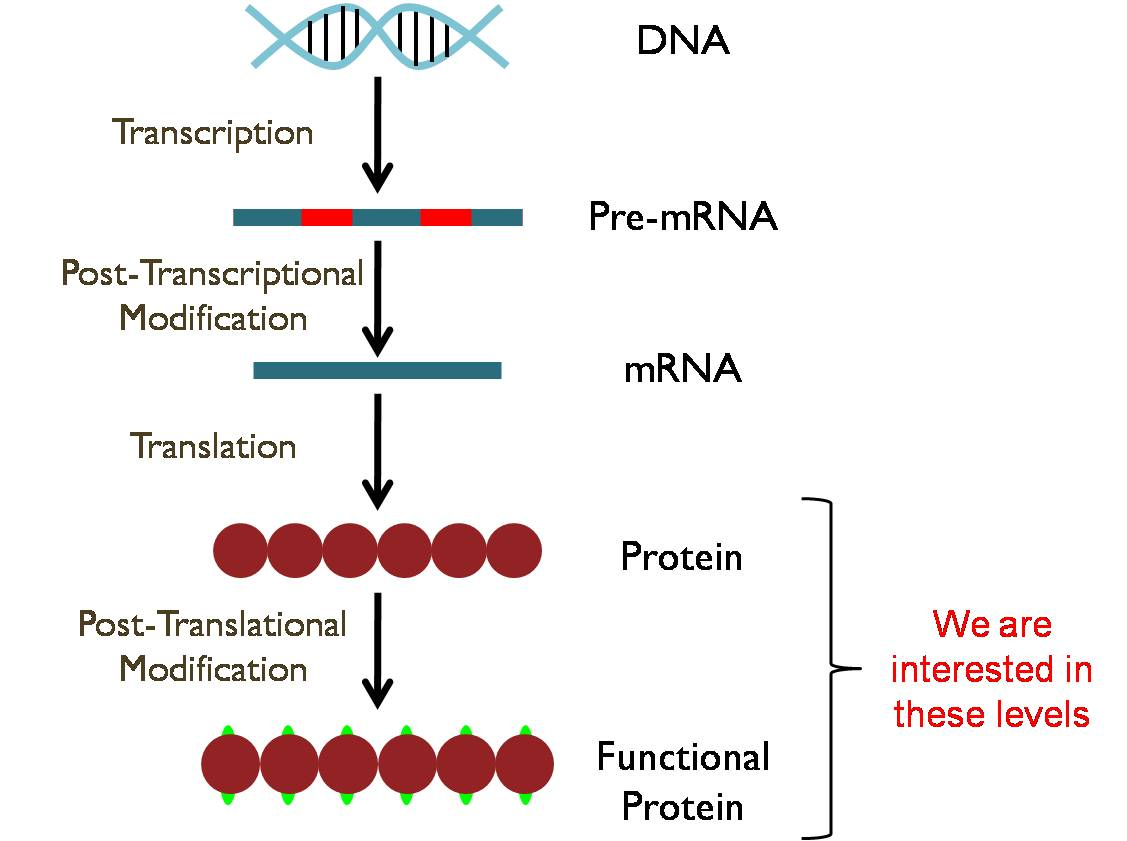
\includegraphics[scale=0.55]{image/processes.jpg}}
\caption{Basic biological processes of producing functional proteins from DNA.}
\label{fig:processes}
\end{figure}

The proteome is the entire complement of proteins expressed by the genome in a cell or tissue or bio-fluid of an organism at a given time under specific conditions \citep{Boehm2007}. The function of a protein corresponds to when and where it is expressed. Proteomic research thus aims to identify and localise many more unknown proteins and their functions. 

There are many ways to study proteins. For example, the physical structure of a protein can be studied by X-ray crystallography~\citep{Blow2002}, protein-protein interactions can be studied using the yeast two-hybrid system~\citep{Fields1989}, and the abundance of an individual protein under a defined condition can be studied using isotopic-labelling. The latter is also labelled \emph{quantitative proteomics}. The use of Multi-dimensional Protein Identification Technology (MudPIT) together with isobaric Tags for Relative and Absolute Quantitation (iTRAQ\textsuperscript{TM}) is just one of the technologies used to measure protein abundance.  

\subsection{Multi-dimensional Protein Identification Technology} \label{subsec:MudPIT}
MudPIT is the process of separating a protein complex or peptide mixture using the properties of amino acids, usually into three orthogonal dimensions~\citep{Washburn2001}. Typically, the first separation is by charge, using \emph{strong cation exchange chromatography} (SCX). This is followed by a second separation by hydrophobicity, using \emph{reversed phase liquid chromatography} (RPLC). The third dimension of separation is by mass, and is carried out by \emph{mass spectrometry} (MS). This reduces the complexity of the sample and enables high throughput protein analysis. Each MudPIT \emph{run} thus comprises these three steps of separation.

MudPIT has some limitations. For example, large variation in signal intensity between different MudPIT runs can make inter-sample comparisons of peptide or protein abundance difficult. This limitation has been resolved by iTRAQ\textsuperscript{TM} labelling, which enables the simultaneous analysis of up to eight distinct protein digests within a single MudPIT run.

\subsection{iTRAQ\textsuperscript{TM} for Protein Quantitation}\label{subsec:iTRAQ}
In its initial format, introduced by \cite{Ross2004}, iTRAQ comprised four isobaric tags, each consisting of a reporter group, balance group and peptide reactive group. The reactive group binds the N-terminus at the start of each peptide, and, if the peptide contains lysine residues (i.e. amino acid), then on the lysine's side chain as well. The m/z values of the four reporter groups range from 114 to 117, with corresponding balance group values that range from 31 to 28. Each of the four tags thus have an identical total m/z value of 145, making them isobaric. This enables identical peptide species, differentially labelled with the four tags, to be indistinguishable with respect to the intact mass of the peptide when selected for MS/MS~\citep{Ross2004}. For MS/MS, the relative abundances are determined from the reporter ion signals at m/z values of 114, 115, 116 and 117 on the \emph{mass spectrum}. A mass spectrum is a graphical representation of the peptides and peptide fragments based on their m/z value and abundances, and is generated for both phases of MS/MS. The four different labels thus allow the simultaneous analysis of four different samples ~\citep{Ross2004}.
  
\begin{figure}[htb]
\centering{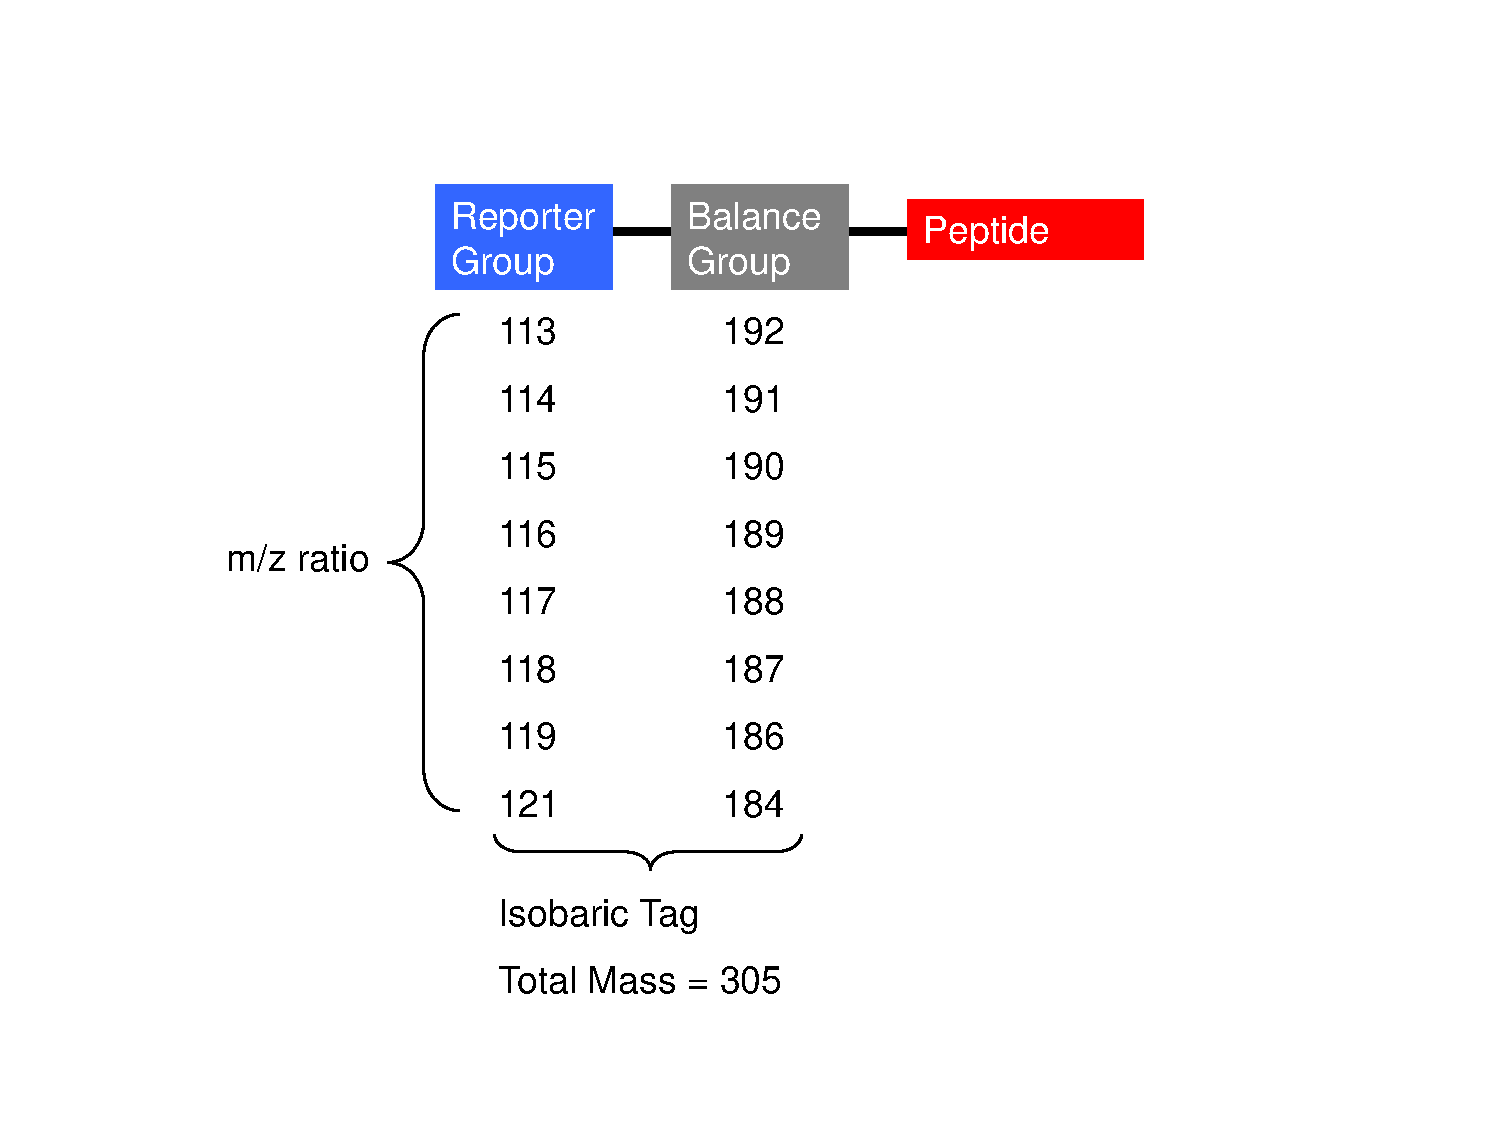
\includegraphics[scale=0.6]{image/iTRAQtags.pdf}}
\caption{Structure of 8-plex-iTRAQ\textsuperscript{TM} tags showing the reporter and balance group masses measured using m/z~\citep{Choe2007}.}
\label{fig:8-plex}
\end{figure}

\cite{Choe2007} described a new multiplexing strategy, based on the same concept as the four-plex iTRAQ\textsuperscript{TM} system, that allows the simultaneous analysis of up to eight distinct protein samples (see Figure~\ref{fig:8-plex}). The scheme involves reporter ion signals located at m/z values of 113, 114, 115, 116, 117, 118, 119 and 121. No label is used for an m/z of 120 because it has the same mass as the phenylalanine immonium ion~\citep{Pierce2008}.  

\section{Overview}
\label{sec:overview}
The main aim of this thesis is to develop general theories for use in two-phase experiments. These can be divided into three main parts, as follows. 

The first part, described in Chapter 2, generalised the decomposition method for two-phase experiments in constructing the ANOVA table. As mentioned by \cite{Brien2011}, the ANOVA tables with the EMS for two-phase experiments are valuable for comparing the properties of different two-phase experimental designs. However, no tool can automatically generate such tables to date. An \textsf{R} package called \textbf{infoDecompuTE} thus is presented that allows the researchers to generate the ANOVA table with EMS by entering any single or two-phase experimental design. This package not only allows researchers to determine whether or not a valid F-test can be conducted from any given design, but also enables them to study the decomposition of the raw data into different strata and sources of variation.

For a given set of design parameters, there are often many ways to allocate the samples collected from the Phase 1 experiment to the blocks of Phase 2 experiment. Chapters 3 and 4 show that the objective function defined can identify the optimal allocation in terms of allowing the administration of a formal test of treatment effects with the highest efficiency factor. The objective function is optimised using a simulated annealing algorithm. Furthermore, the objective function presented can be used to optimise the two-phase design, where the Phase 1 experiment uses a completely randomised design and block design, while the Phase 2 experiment has a randomised block design. This type of two-phase experiment structure is typically used for the high-throughput biotechnology experiment. Additionally, an improved and more efficient version of the SA is presented.

Finally, Chapter 5 describes a method used to estimate the variance components and the EDF for the two-phase experiments. The restricted maximum likelihood method is described in estimating the variance components of the two-phase experiment with non-orthogonal block structures. EDF, computed from different variance component estimates, is then used to compare the different optimal two-phase designs found in Chapters 3 and 4. These specific examples are used to clarify the properties of different candidate designs and further develop a general theory of two-phase experiments.  


\bibliographystyle{apalike}
\bibliography{ref}

\end{document}
